\chapter{Architektura a implementace aplikace}

\section{Serverová část}

Serverová část aplikace je naprogramovaná v jazyce C\# s použitím 
frameworku ASP .NET Core. Je rozdělena do těchto projektů:

\subsection{Data}

Tento projekt se stará primárně o komunikaci s databází, pro tento účel jsme použili ORM framework Entity Framework Core. 

Ve složce Models jsou třídy reprezentující databázové entity. Každá z entit pak v databázi představuje jednu tabulku. V aplikaci jsme použili tyto entity:

\begin{table}[ht]
	\centering
	\begin{tabular}{| l | p{9cm} |}
		\hline
		Název entity & reprezentovaný objekt \\
		\hline \hline
		Course & kurz \\ \hline
		CourseFile & nějaký soubor sdílený v kurzu \\ \hline
		CourseMember & členství uživatele v daném kurzu. 
		K této entitě se pak vážou všechny známky a odeslané testy. \\ \hline
		CourseTest & test v kurzu \\ \hline
		ForumPost & příspěvek ve fóru k danému kurzu \\ \hline
		Grade & známku kterou student obdržel (kromě známek z testů) \\ \hline
		Person & uživatele aplikace \\ \hline
		TestQuestion & 1 otázku v testu \\ \hline
		TestSubmission & test s odpověďmi odeslaný uživatelem \\ \hline
		TestSubmissionAnswer & odpověď k dané otázce v testu \\
		\hline
	\end{tabular}
\end{table}

\newpage

\begin{figure}
	\centering
	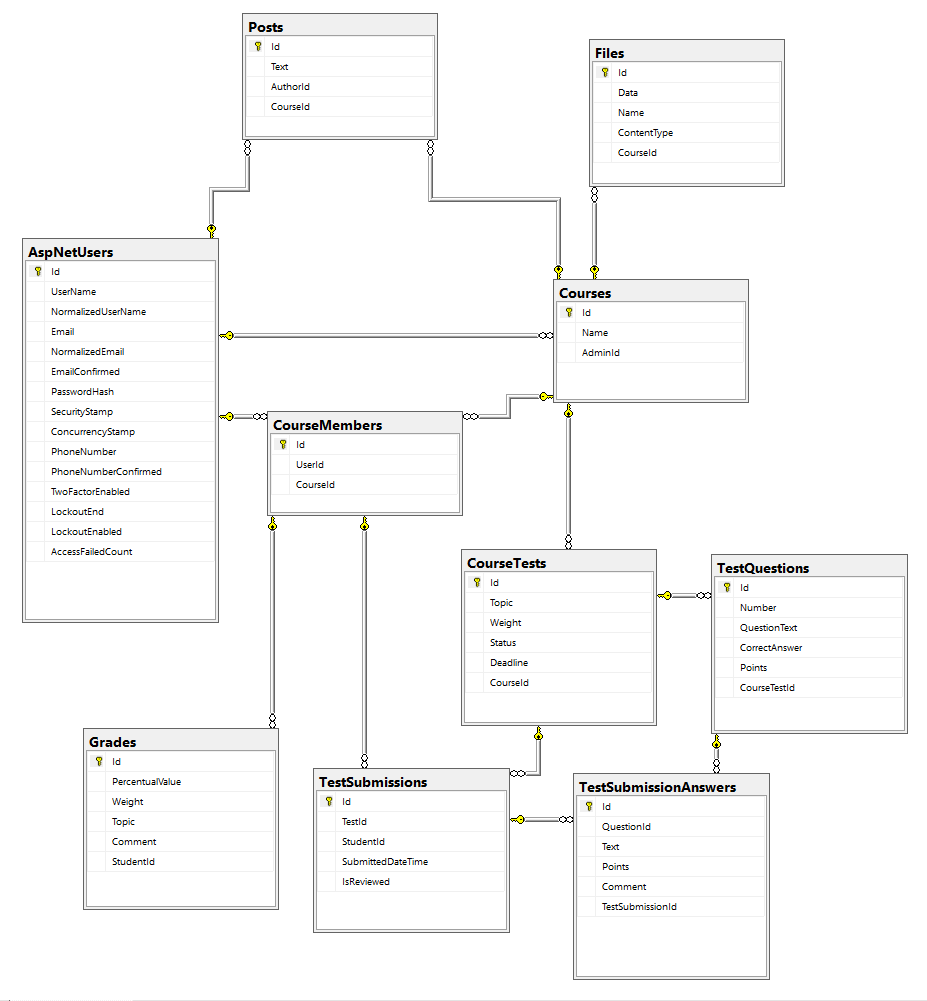
\includegraphics[width=\textwidth]{db_model.PNG}
	\caption{Databázový model aplikace}
\end{figure}

\newpage

Pro ilustraci uvedeme kód třídy Course:

\begin{lstlisting}
public class Course : IGuidIdObject
{
	public Course()
	{
		Members = new List<CourseMember>();
		Files = new List<CourseFile>();
		Tests = new List<CourseTest>();
		ForumPosts = new List<ForumPost>();
	}
	
	public Course(string name, Person admin) : this()
	{
		Name = name;
		Admin = admin;
	}
	
	/// <summary>
	/// identifier of the couse
	/// </summary>
	[DatabaseGenerated(DatabaseGeneratedOption.Identity)]
	[Key]
	public Guid Id { get; set; }
	
	/// <summary>
	/// name of the course
	/// </summary>
	[Required]
	public string Name { get; set; }
	
	...
\end{lstlisting}

Vidíme, že každá entita obsahuje veřejné vlastnosti (public properties) s gettery a settery. Tyto vlastnosti budou v databázové tabulce reprezentovány jako sloupce. Některé z nich (jako např. Id) obsahují ještě doplňující atributy, ty slouží k upřesnění informací o dané vlastnosti. Například atribut [Key] určuje, že tato vlastnost bude v databázi primární klíč, atribut [Required] určuje, že daný sloupec bude v tabulce u všech záznamů povinný (tedy hodnoty budou NOT NULL).
Dále musí každá entita obsahovat konstruktor bez parametrů.

Vazby mezi entitami jsou reprezentované pomocí tzv. navigačních vlastností. V případě, že chceme vytvořit vazbu typu one-to-many mezi entitami A a B, stačí do vlastností třídy A přidat kolekci objektů typu B, a naopak do třídy B vlastnost typu A. Framework pak při provádění migrace vytvoří v databázové tabulce entity B vytvoří sloupec s cizím klíčem, který bude obsahovat identifikátor entity A, ke které patří.

V aplikaci je vazba one-to-many použita mimo jiné mezi entitami Course a CourseTest, a to tak, že každý test je obsažen v právě jednom kurzu, a v daném kurzu může být N testů.
Kód pak tedy vypadá takto: Ve třídě Course je kolekce objektů typu CourseTest

\begin{lstlisting}
/// <summary>
/// tests in this course
/// </summary>
public ICollection<CourseTest> Tests { get; set; }
\end{lstlisting}

Ve třídě CourseTest je pak vlastnost typu Course

\begin{lstlisting}
/// <summary>
/// course that contains this test
/// </summary>
[Required]
public Course Course { get; set; }
\end{lstlisting}

Po provedení databázové migrace (viz. dále) se v tabulce CourseTest vytvoří sloupec CourseId s cizím klíčem, který odkazuje na identifikátor kurzu (tzn. vlastnost Course.Id).

Také si můžeme všimnout, že všechny entity (kromě entity Person) implementují rozhraní IGuidObject. To je jednoduché rozhraní, které obsahuje pouze jednu vlastnost -- Id typu Guid. Tímto máme zajištěnou jednotu identifikátorů, tedy že všechny entity, které toto rozhraní implementují, budou mít identifikátor typu Guid.

\begin{lstlisting}
/// <summary>
/// interface for object with <see cref="Guid"/> identifier
/// </summary>
public interface IGuidIdObject
{
	/// <summary>
	/// identifier of the object
	/// </summary>
	Guid Id { get; set; }
}
\end{lstlisting}


Typ Guid jsme zvolili hlavně z toho důvodu, že vestavěné tabulky frameworku (např. Identity) mají také řetězcové identifikátory. Navíc se pak zjednoduší práce ve frontend části (není potřeba parsovat string na int např. v klientské části při práci s URL). Tyto identifikátory generuje databáze, takže je zajištěno, že jsou unikátní.
Další možnost by byla použít jako identifikátor číslo (např. typ int), ale vzhledem k výše uvedeným argumentům je typ Guid v tomto případě lepší možnost.

Dále se v projektu nacházejí také rozhraní ICourseReferenceObject a ICourseMemberReferenceObject, která slouží k tomu, abychom mohli dále v aplikaci jednotně pracovat s objekty, které mají referenci na entitu Course, resp. CourseMember. Tato rozhraní implementují pouze nějaké entity.

Třída CMSDbContext reprezentuje databázový kontext této aplikace. Každý objekt typu DbSet pak představuje jednu databázovou tabulku. Ve třídě je CMSDbContext tedy kolekce typu DbSet pro každou z entit.

\begin{lstlisting}
public DbSet<Grade> Grades { get; set; }

public DbSet<Course> Courses { get; set; }

...
\end{lstlisting}

Jediná výjimka je entita Person, která dědí ze třídy IdentityUser, a jejíž DbSet je nakonfigurovaný ve frameworku. 

V programu pak dále používáme ke komunikaci s databází pouze třídu CMSDbContext a objekty typu DbSet. Třída DbSet<TEntity> implementuje rozhraní IQueryable<TEntity>, takže na ni lze použít LINQ. Takže pokud bychom chtěli například vybrat všechny kurzy, jejiž jméno začíná na písmeno C, pak stačí použít následující LINQ dotaz
\begin{lstlisting}
dbContext.Courses.Where(course => course.Name.StartsWith("C"))
\end{lstlisting}
kde proměnná dbContext je instance třídy CMSDbContext.

Ve třídě CMSDbContext je také metoda ConfigureForeignKeys, která provede konfiguraci cizích klíčů v aplikaci. Všechny políčka s cizími klíči jsou v databázi povinné (tzn. NOT NULL), to je zajištěno pomocí atributu [Required] daných vlastností. Nastavením DeleteBehavior.Restrict u cizích klíčů zajistíme, že databáze zůstane v konzistentním stavu. Pokud bychom tedy chtěli smazat entitu, pak na ni nesmí pomocí cizích klíčů odkazovat jiné entity. V opačném případě program při zavolání metody SaveChanges() na databázovém kontextu vyhodí výjimku.

V programu je dále složka Migrations. Při vývoji byl použit princip Code first, tedy že v kódu specifikujeme entity pomocí klasických tříd. Framework se pak postará o vytvoření databázových tabulek z tohoto kódu.

Pokud tedy nějak změníme některou z entit (to může být např. přidání vlastnosti, změna jména vlastnosti, apod.), pak pomocí ORM můžeme vygenerovat soubor popisující tzv. databázovou migraci, která slouží k aplikaci změn z kódu do databáze. Ke každé migraci se vygeneruje jeden soubor, který obsahuje popis změn, které se později provedou v databázi.

K vytváření migrací jsem použijeme nástroj CLI tools for Entity Framework Core. https://docs.microsoft.com/cs-cz/ef/core/cli/dotnet. Pro vygenerování migrace ze změn v kódu použijeme příkaz:

TO-Do: přesunout přesný příkaz jinam

\begin{lstlisting}
dotnet ef migrations add {migration_name} 
--project CourseManagementSystem.Data 
--startup-project CourseManagementSystem.API
\end{lstlisting}

Tímto se vytvoří soubor popisující změny v migraci, ale databáze zatím zůstala beze změny. Tento soubor obsahuje třídu, jenž dědí ze třídy Migration a obsahuje metody Up a Down. V metodě Up je popis změn, které se provedou při aplikaci této migrace, naopak v metodě Down je popis změn, které se provedou v případě odstranění migrace.

Jako příklad si můžeme představit migraci, která obsahuje přidání vlastnosti ScoreWeight k entitě CourseTest (tato vlastnost popisuje váhu testu).
Vygenerovaný kód migrace vypadá takto:

\begin{lstlisting}
public partial class TestWeight_added : Migration
{
	protected override void Up(MigrationBuilder migrationBuilder)
	{
		migrationBuilder.AddColumn<int>(
		name: "ScoreWeight",
		table: "CourseTests",
		nullable: false,
		defaultValue: 0);
	}
	
	protected override void Down(MigrationBuilder migrationBuilder)
	{
		migrationBuilder.DropColumn(
		name: "ScoreWeight",
		table: "CourseTests");
	}
}
\end{lstlisting}

TO-DO: přesunout syntaxi příkaz jinam

Pro promítnutí změn do databáze následně použijeme příkaz:

\begin{lstlisting}
dotnet ef database update 
--project CourseManagementSystem.Data 
--startup-project CourseManagementSystem.API
\end{lstlisting}

Tímto tedy dojde k změnám v databázi (v našem příkladu se vytvoří sloupec ScoreWeight v tabulce CourseTests).

V obou příkazech je potřeba specifikovat cílový a startup projekt. Cílový projekt je ten, který obsahuje databázový kontext a entity naší aplikace (v tomto případě projekt Data). Naopak startup projekt je projekt, který je spouštěný frameworkem, což je potřeba pro získání konfiguračních informací o projektu, jako je například connection string do naší databáze.

\newpage

\subsection{Services}
V tomto projektu se nachází pomocné služby pro komunikaci s databází. 

Jako základ pro všechny služby slouží abstraktní třída DbService, která obsahuje referenci na databázový kontext aplikace a jedinou metodu CommitChanges(). Ta slouží k uložení změn provedených v databázovém kontextu do databáze. 

To je potřeba, protože k uložení změn do databáze dojde až tehdy, když na databázovém kontextu zavoláme metodu SaveChanges(). Pokud bychom tedy například do databázového kontextu něco uložili (např. takto: 
\begin{lstlisting}
dbContext.Grades.Add(new Grade())
\end{lstlisting})
a nezavolali metodu dbContext.SaveChanges(), data by se neuložila.

\begin{lstlisting}
/// <summary>
/// class representing base database service
/// </summary>
public abstract class DbService : IDbService
{
	/// <summary>
	/// context of the CMS database
	/// </summary>
	protected readonly CMSDbContext dbContext;
	
	/// <summary>
	/// construct a new database service
	/// </summary>
	/// <param name="dbContext">CMS database context</param>
	protected DbService(CMSDbContext dbContext)
	{
		this.dbContext = dbContext;
	}
	
	/// <inheritdoc/>
	public void CommitChanges()
	{
		dbContext.SaveChanges();
	}
}
\end{lstlisting}

Tato třída implementuje rozhraní IDbService, které obsahuje pouze metodu CommitChanges().

Dále jsou ve složce Interfaces rozhraní pro další služby, ty jsou rozdělené podle entit (typicky máme pro jednu entitu jednu službu). Všechny tyto rozhraní také implementují rozhraní IDbService. 

Například rozhraní ICourseService (slouží pro práci s kurzy) vypadá takto:
\begin{lstlisting}
public interface ICourseService : IDbService
{
	/// <summary>
	/// get course by its id
	/// </summary>
	/// <param name="courseId">identifier of the course</param>
	/// <returns></returns>
	Course GetById(string courseId);
	
	/// <summary>
	/// archive course by its id
	/// </summary>
	/// <param name="courseId">id of the course to delete</param>
	void ArchiveById(string courseId);
	
	/// <summary>
	/// add the course into the database
	/// </summary>
	/// <param name="course">course to add</param>
	void AddCourse(Course course);
	...
\end{lstlisting}

Ve složce Implementations jsou potom implementace těchto rozhraní. Můžeme vidět, že všechny implementace dědí ze třídy DbService, a zároveň také tranzitivně implementují IDbService.

Například třída CourseService, která implementuje rozhraní ICourseService vypadá takto:

\begin{lstlisting}
public class CourseService : DbService, ICourseService
{
	public CourseService(CMSDbContext dbContext) : base(dbContext)
	{ }
	
	/// <inheritdoc/>
	public void ArchiveById(string courseId)
	{
		Course c = GetById(courseId);
		c.IsArchived = true;
	}
	
	/// <inheritdoc/>
	public Course GetById(string courseId)
	{
		return dbContext.Courses.FindById(courseId);
	}
	
	/// <inheritdoc/>
	public void AddCourse(Course course)
	{
		dbContext.Courses.Add(course);
	}
	...
\end{lstlisting}

Vidíme, že služby typicky pracují s databázovým kontextem a s daty (vyhledávání, mazání, apod.).
Dále si můžeme všimnout, že v žádné metodě se neukládájí změny do databáze (tzn. volání metody CommitChanges()). To je z toho důvodu, že ve vyšších vrstvách aplikace (např. API) v jedné metodě často voláme několik služeb, příp. několik metod z jedné služby. 
Pokud bychom v metodách služeb přímo ukládali změny do databáze (metoda CommitChanges()), pak bychom se mohli lehce dostat to nekonzistentního stavu. To například tak, že při volání několika služeb v rámci jedné metody by 
mohla některá ze služeb vyhodit výjimku, nicméně všechny služby zavolané předtím by už data uložily.

Je na zodpovědnosti volajícího provést uložení změn do databáze, tedy zavolat metodu CommitChanges(), což je typicky poslední příkaz v dané metodě.
Tím jsme tedy zajistili konzistenci dat - buď se do databáze uloží všechny změny provedené v databázovém kontextu, nebo žádné.

Dále si můžeme všimnout, že ve službách pracujeme s identifikátory typu string, ale v databázi používáme typ Guid. To je z toho důvodu, že ve vyšších vrstvách aplikace se pohodlněji pracuje se stringy (např. často dostáváme ID jako URL parametr). Převod mezi typy string a Guid pak řešíme ve službách.

Ve složce Extensions jsou pak pomocné metody pro práci s některými třídami.

Ve třídě DbSetExtensions se nachází extension metody pro třídu DbSet<T>. Vybereme si například metodu GetCourseIdOf, ta slouží k získání ID kurzu, ke kterému daný objekt, jenž má referenci na entitu Course, patří.
\begin{lstlisting}
/// <summary>
/// get id of <see cref="Data.Models.Course"/> that the object belongs to
/// </summary>
/// <typeparam name="T">type of items</typeparam>
/// <param name="dbSet">database set</param>
/// <param name="objectId">identifier of the object we look for in <paramref name="dbSet"/></param>
/// <returns></returns>
public static string GetCourseIdOf<T>(this DbSet<T> dbSet, string objectId) where T : class, ICourseReferenceObject, IGuidIdObject
{
	return dbSet.Include(item => item.Course)
		.Single(item => item.Id.ToString() == objectId)
		.Course.Id.ToString();
}
\end{lstlisting}

Vidíme, že toto je jeden z příkladů použití rozhraní ICourseReferenceObject, které se nachází v projektu Data.

V projektu též máme rozhraní ICourseReferenceService, to implementují všechny služby, jejichž entity logicky patří k nějakému kurzu. Rozhraní obsahuje jedinou metodu GetCourseIdOf(string objectId), která získá ID kurzu, ke kterému daná entita patří. V implementaci této metodu pak typicky používáme extension metodu GetCourseIdOf pro třídu DbSet<T>. Například ve třídě CourseTestService vypadá implementace takto:

\begin{lstlisting}
public string GetCourseIdOf(string objectId)
{
	return dbContext.CourseTests.GetCourseIdOf(objectId);
}
\end{lstlisting}

Podobně je v projektu i rozhraní ICourseMemberReferenceService, které používají služby, jejichž entity mají referenci na třídu CourseMember.

Použitím služeb jsme odstranili duplikátní kód (např. hledání kurzu podle ID se používá na několika místech ve vyšších vrstvách), a extrahovali některé složitější dotazy do samostatných metod. To je výhodné hlavně z toho důvodu, že je pak můžeme nezávisle otestovat. Další výhoda je, že vyšší vrstvy jsou odstíněny od použití ORM (a databázového kontextu), pouze volají tyto služby.

Dále si můžeme všimnout, že ve službách používáme při komunikaci s databázovým kontextem tzv. Eager loading (pomocí metod Include()). To znamená, že data databázových entit které daná entita referencuje, se při výchozím chování nenačtou (pokud nepoužijeme metodu Include), tzn. budou mít hodnotu NULL.

Například pro získání testu s otázkami můžeme použít tento příkaz:
\begin{lstlisting}
dbContext.CourseTests
	.Include(test => test.Questions)
\end{lstlisting}
Pokud bychom volání metody Include() vynechali, tak by se data otázek nenačetla.

\newpage

\subsection{API}
V této části se nachází popis projektu API, které slouží pro komunikaci klientské části se serverovou.

\subsubsection*{Controllers}
Controllery slouží primárně ke zpracování HTTP požadavků. Vidíme, že Controller je klasická C\# třída, jež dědí ze třídy ControllerBase. Ve většině případů obsahuje reference na služby (jako privátní položky).

\begin{lstlisting}
[Route("api/[controller]")]
[ApiController]
[Authorize]
public class CoursesController : ControllerBase
{
	private readonly IHttpContextAccessor httpContextAccessor;
	private readonly ICourseService courseService;
	private readonly IPeopleService peopleService;
	private CourseTestFilter courseTestFilter;
	
	public CoursesController(IHttpContextAccessor httpContextAccessor, ICourseService courseService, IPeopleService peopleService)
	{
		this.httpContextAccessor = httpContextAccessor;
		this.courseService = courseService;
		this.peopleService = peopleService;
		courseTestFilter = new CourseTestFilter();
	}
	...
\end{lstlisting}

Jednotlivé Controllery pak obsahují veřejné metody, jež odpovídají HTTP endpointům.

Například následující metoda slouží k získaní všech členů daného kurzu.
\begin{lstlisting}
/// <summary>
/// get all course members
/// </summary>
/// <param name="id">Id of the course</param>
[HttpGet("{id}/members")]
[AuthorizeCourseAdminOf(EntityType.Course, "id")]
public IEnumerable<CourseMemberOrAdminVM> GetAllMembers(string id)
{
	var people = courseService.GetMembersWithUsers(id);
	return people.Select(cm => new CourseMemberOrAdminVM(cm.Id.ToString(), cm.User.UserName, cm.User.Email));
}
\end{lstlisting}

Vidíme, že je tedy označená atributem HttpGet, který zároveň obsahuje URL, přes kterou lze tuto metodu zavolat. V tomto případě je URL suffix "\{id\}/members". Položka Id označuje parametr, jenž má stejnou hodnotu jako proměnná id (parametr metody). Tento suffix se připojí za URL daného Controlleru, a tím získáme celou URL k zavolání této metody. V našem případě dostaneme
\newline
"http://host/api/courses/course-id/members", kde course-id je identifikátor příslušného kurzu a host označuje URL serveru, na kterém aplikace běží. Pokud máme aplikaci spuštěnou lokálně, pak by hodnota měla být localhost:5001. Při HTTP GET dotazu na tuto URL by tedy aplikace zavolala tuto metodu, a vrátila data.

Metoda dále obsahuje atribut určený k autorizaci, pomocí něhož ověříme, že klient má dostatečná práva. V tomto případě povolíme zavolat metodu pouze administrátorům daného kurzu.

V těle metody pak zavoláme konkrétní službu, která typicky pracuje s databází. Tato služba nám vrátí data (v tomto případě všechny členy daného kurzu), které potom namapujeme na objekty typu ViewModel, a ty vrátíme.

\vspace{\baselineskip}

V dalším příkladu máme metodu, která slouží k vytvoření nového kurzu.
\begin{lstlisting}
/// <summary>
/// create new course
/// </summary>
[HttpPost("create")]
public void Create(AddCourseVM courseVM)
{
	string currentUserId = httpContextAccessor.HttpContext.GetCurrentUserId();
	Person admin = peopleService.GetById(currentUserId);
	Course createdCourse = new Course(courseVM.Name, admin);
	
	courseService.AddCourse(createdCourse);
	
	courseService.CommitChanges();
}
\end{lstlisting}
Tato metoda je označena atributem HttpPost, který opět obsahuje URL suffix. Pokud bychom tedy chtěli zavolat tuto metodu, pak je potřeba provést HTTP POST požadavek na URL
\newline
"http://host/api/courses/create", který v těle obsahuje JSON objekt typu AddCourseVM. Framework pak provede deserializaci objektu, a objekt (instanci třídy AddCourseVM) předá jako parametr do této metody.

V těle metody následně vytvoříme nový objekt kurzu, a pomocí příslušné služby (v tomto případě CourseService) jej přidáme k existujícím kurzům. Můžeme si všimnout, že na konci metody voláme metodu CommitChanges(), která změny zapíše do databáze.

\subsubsection*{ViewModels}
\label{serverVM}

ViewModels reprezentují objekty pro komunikaci mezi Frontend a Backend částí (konkrétně mezi Frontend službami a API). Tedy např. při GET dotazu vrací příslušný Controller objekt (příp. objekty) typu ViewModel. Stejně tak při POST dotazu posílá klient v těle požadavku objekt typu ViewModel.

Příklad:
\begin{lstlisting}
/// <summary>
/// viewmodel for submitting a test
/// </summary>
public class SubmitTestVM
{
	public SubmitTestVM()
	{
	}
	
	public SubmitTestVM(string testId, string testTopic, bool isSubmitted, IEnumerable<SubmissionAnswerVM> answers, bool isTestGraded)
	{
		TestSubmissionId = testId;
		TestTopic = testTopic;
		Answers = answers;
		IsSubmitted = isSubmitted;
		IsTestGraded = isTestGraded;
	}
	
	/// <summary>
	/// id of the test submission
	/// </summary>
	[RequiredWithDefaultErrorMessage]
	public string TestSubmissionId { get; set; }
	
	/// <summary>
	/// topic of the test
	/// </summary>
	[RequiredWithDefaultErrorMessage]
	public string TestTopic { get; set; }
	
	/// <summary>
	/// check if the test has already been submitted
	/// </summary>
	public bool IsSubmitted { get; set; }
	...
\end{lstlisting}

Tento ViewModel reprezentuje data odevzdávaného testu. Vidíme, že ViewModely jsou typicky veřejné třídy s veřejnými vlastnostmi. Dále vidíme, že ViewModel má veřejný bezparametrový konstuktor, ten je volán při deserializaci dat.

Také si můžeme všimnout, že u některé vlastnosti ještě obsahují doplňující atributy (např. atribut [RequiredWithDefaultErrorMessage] u vlastnosti TestTopic). Tyto atributy slouží primárně k validaci dat.

Ve ViewModelech poměrně často používáme dědičnost, podobně jako v tomto příkladu.
\begin{lstlisting}
/// <summary>
/// base viewmodel for course tests
/// </summary>
public abstract class BaseCourseTestVM
{
	protected BaseCourseTestVM()
	{
	}
	
	protected BaseCourseTestVM(int weight, string topic, ...)
	{
		...
	}
	
	/// <summary>
	/// weight of the score from the test (e.g. test of weight 2 has twice bigger impact on overall score than test of weight 1)
	/// </summary>
	[PositiveIntValue]
	public int Weight { get; set; }
	
	/// <summary>
	/// topic of the test
	/// </summary>
	[RequiredWithDefaultErrorMessage]
	public string Topic { get; set; }

	...
}

/// <summary>
/// viewmodel for adding a course test
/// </summary>
public class AddCourseTestVM : BaseCourseTestVM
{
	public AddCourseTestVM() : base()
	{ }
}

/// <summary>
/// viewmodel representing a test in a course
/// </summary>
public class CourseTestDetailsVM : BaseCourseTestVM
{
	public CourseTestDetailsVM() : base()
	{ }
	
	public CourseTestDetailsVM(string id, string topic, int scoreWeight, ...)
	: base(scoreWeight, topic, ...)
	{
		Id = id;
		Status = testStatus;
	}
	
	/// <summary>
	/// id of the test
	/// </summary>
	[RequiredWithDefaultErrorMessage]
	public string Id { get; set; }
	
	/// <summary>
	/// status of the test
	/// </summary>
	public TestStatus Status { get; set; }
}
\end{lstlisting}
Chceme vytvořit alespoň dva ViewModely, jejichž struktura je velmi podobná a liší se jen přítomností několika málo doplňujících vlastností. Řešením je vytvořit Base třídu, která obsahuje všechny společné vlastnosti. Pro konkrétní ViewModely poté můžeme vytvořit třídy, které dědí z této rodičovské třídy, a obsahují již pouze doplňující vlastnosti.

Ve výše uvedeném příkladu máme tedy třídu BaseCourseTestVM, a od ní dědí třídy AddCourseTestVM a CourseTestDetailsVM. Tyto ViewModely slouží k přidání nového testu, resp. získání informací o daném testu.

Vidíme, že vlastnosti Id a Status se nachází pouze ve třídě CourseTestDetailsVM. Toto dává smysl, jelikož při vytváření testu ještě neznáme jeho identifikátor (objekt ještě není uložený v databázi).
Podobně je to i se stavem (vlastnost Status), jelikož ten bude při vytváření vždy nastaven na New.

Bylo by samozřejmě možné oba ViewModely sloučit do jedné třídy se všemi vlastnostmi. Toto řešení je ale podle mého názoru velmi matoucí, jelikož vlastnosti Id a Status jsou při vytváření testu zbytečné.

\subsubsection*{Atributy určené k validaci}

V programu používáme několik vlastních atributů, určených k validaci dat, ty se nachází ve složce Validation/Attributes.
Atribut je klasická C\# třída, která dědí ze třídy System.Attribute. Její název obvykle končí suffixem "Attribute".

Příklady:
\begin{lstlisting}
/// <summary>
/// Validation attribute that marks this value as required
/// <br/>
/// if validation fails <see cref="defaultErrorMessage"/> is displayed
/// </summary>
public class RequiredWithDefaultErrorMessageAttribute : RequiredAttribute
{
	/// <summary>
	/// default error message displayed ({0} is replaced by the field name that this attribute belongs to)
	/// </summary>
	public const string defaultErrorMessage = "The field {0} is required";
	
	public RequiredWithDefaultErrorMessageAttribute()
	{
		ErrorMessage = defaultErrorMessage;
	}
}

/// <summary>
/// Validation attribute that validates if the double value is non-negative (e.g. >=0)
/// <br/>
/// if validation fails <see cref="defaultErrorMessage"/> is displayed
/// </summary>
public class NonNegativeDoubleValueAttribute : RangeAttribute
{
	/// <summary>
	/// default error message displayed ({0} is replaced by the field name that this attribute belongs to)
	/// </summary>
	public const string defaultErrorMessage = "The field {0} must be non-negative";
	
	public NonNegativeDoubleValueAttribute() : base(0, double.MaxValue)
	{
		ErrorMessage = defaultErrorMessage;
	}
}
\end{lstlisting}

\begin{itemize}
\item NonNegativeDoubleValueAttribute -- Tento atribut validuje, že vlastnost typu double, ke které patří, je nezáporné číslo. V případě, že tomu tak není, nastavíme výchozí chybovou hlášku "The field \{0\} must be non-negative", kde \{0\} je název vlastnosti, ke které atribut patří.

\item RequiredWithDefaultErrorMessageAttribute -- Tento atribut dědí z atributu RequiredAttribute. Pokud má příslušná vlastnost hodnotu null, nebo se jedná o řetězec, který je prázdný, nebo složený pouze z bílých znaků, tak validace selže. Atribut RequiredWithDefaultErrorMessage pak slouží jen k přidání výchozí chybové hlášky "The field \{0\} is required", v případě, že validace selže.

\end{itemize}

Dále jsou v aplikaci ještě použité atributy NonNegativeIntValueAttribute a PositiveIntValueAttribute.


\subsubsection*{Obsluha chyb}

V případě, že nastane chyba při deserializaci dat (např. klient pošle v těle POST dotazu nevalidní data), tak framework vyhodí výjimku a vrátí objekt, který popisuje chybu. \url{https://docs.microsoft.com/en-us/aspnet/core/web-api/?view=aspnetcore-5.0#automatic-http-400-responses}

Pokud nastane chyba při obsluze dotazu (např. klient se pomocí GET dotazu pokusí získat informace o nějaké již smazané entitě), pak v programu vyhodíme výjimku. Všechny výjimky jsou pak zachyceny třídou ErrorHandlerController, která funguje jako obecný Error handler.
Toto je nakonfigurováno v metodě Configure(), jenž se nachází ve třídě Startup.
\begin{lstlisting}
/// <summary>
/// controller for error handling
/// </summary>
[ApiExplorerSettings(IgnoreApi = true)]
public class ErrorHandlerController : ControllerBase
{
	private const string generalErrorText = "An error occurred while processing the request.";
	
	/// <summary>
	/// handle runtime error
	/// </summary>
	/// <returns></returns>
	[Route("errorHandler")]
	public IActionResult HandleError()
	{
		var context = HttpContext.Features.Get<IExceptionHandlerFeature>();
		var exception = context.Error; // thrown exception
		
		var errorDescription = new Dictionary<string, string[]>
		{
			{ "Request failed", new string[] { generalErrorText } }
		};
		
		var errorsVM = new ErrorsDictionaryVM(errorDescription);
		return BadRequest(errorsVM);
	}
}
\end{lstlisting}
Metoda HandleError tedy nastaví kód odpovědi na 400 Bad Request, a vrátí objekt typu ErrorsDictionaryVM.
Ten v tomto případě obsahuje obecnou hlášku "An error occurred while processing the request."

\subsubsection*{Autorizace}

V programu máme také server-side autorizaci. Ta slouží k ověření toho, jestli je uživatel oprávněný provést danou akci. Základní entitou pro autorizaci je kurz (entita Course). V aplikaci tedy vždy ověřujeme, jestli je aktuální uživatel administrátor (příp. člen) kurzu, ke kterému se vztahuje daná entita (např. CourseTest).

K tomuto účelu používáme autorizační atributy, které se nachází ve složce Auth/Attributes. 
Abstraktní třída CourseBasedAuthorizeFilter slouží jako rodičovská třída pro všechny filtry, založené na autorizaci pomocí kurzů.

\begin{lstlisting}
/// <summary>
/// filter for authorization based on <see cref="Data.Models.Course"/> related entity
/// </summary>
public abstract class CourseBasedAuthorizeFilter : IAuthorizationFilter
{
	/// <summary>
	/// type of the course related entity
	/// </summary>
	private readonly EntityType entityType;
	
	/// <summary>
	/// name of the field in HTTP route that contains the id of the entity
	/// </summary>
	private readonly string entityIdFieldName;
	
	/// <summary>
	/// factory for <see cref="Services.Interfaces.ICourseReferenceService"/> services
	/// </summary>
	private readonly ICourseReferenceServiceFactory courseReferenceServiceFactory;

	/// <inheritdoc/>
	public void OnAuthorization(AuthorizationFilterContext context)
	{
		if (context.HttpContext.User.Identity.IsAuthenticated)
		{
			string currentUserId = context.HttpContext.GetCurrentUserId();
			string objectId = context.HttpContext.Request
				.RouteValues[entityIdFieldName].ToString();
			
			var service = courseReferenceServiceFactory
				.GetByEntityType(entityType);
			string courseId = service.GetCourseIdOf(objectId);
			
			if (IsAuthorized(currentUserId, courseId, entityType, objectId))
			{
				// authorization passed -> proceed to controller
				return;
			}			
		}
		context.Result = new UnauthorizedResult();
	}
	
	/// <summary>
	/// check if the user is authorized to access the course related entity
	/// </summary>
	/// ...
	protected abstract bool IsAuthorized(string currentUserId, string courseId, EntityType entityType, string entityId);
	
	...
}
\end{lstlisting}

Vidíme, že tato třída obsahuje typ entity (proměnná entityType), pomocí které provádíme autorizaci. Dále také název proměnné v URL, která obsahuje identifikátor této entity. 

Metoda OnAuthorization se automaticky zavolá při autorizaci. V této metodě nejprve zkontrolujeme, že uživatel je přihlášený, poté získáme jeho ID (přes HttpContext) a ID dané entity. Poté získáme identifikátor kurzu, ke kterému daná entita logicky patří. Zde využíváme toho, že všechny služby implementují rozhraní ICourseReferenceService. 
Dále zjistíme, jestli má uživatel dostatečná práva. K tomuto účelu slouží abstraktní metoda IsAuthorized. 

Jedná se o využití návrhového vzoru Template method, kdy implementaci této metody necháme na třídách, které dědí z CourseBasedAuthorizeFilter. 
Společné kroky autorizace nicméně implementujeme v této (rodičovské) třídě.

Pokud zjistíme, že uživatel nemá dostatečná práva, pak pouze vrátíme UnauthorizedResult, a požadovaná akce se neprovede.

Dále ještě potřebujeme v aplikaci mechanismus, který nám podle enumu EntityType vrátí příslušnou službu. K tomuto účelu používáme třídu CourseReferenceServiceFactory.
\begin{lstlisting}
/// <summary>
/// factory for <see cref="ICourseReferenceService"/>
/// </summary>
public class CourseReferenceServiceFactory : ICourseReferenceServiceFactory
{
	...
	
	private readonly IReadOnlyDictionary<EntityType, ICourseReferenceService> dataServices;
	
	public CourseReferenceServiceFactory(ICourseAdminService courseAdminService, ICourseMemberService courseMemberService, ...)
	{
		dataServices = new Dictionary<EntityType, ICourseReferenceService>
		{
			[EntityType.CourseMember] = courseMemberService,
			[EntityType.CourseAdmin] = courseAdminService,
			[EntityType.CourseTest] = courseTestService,
			...
		};
	}
	
	/// <inheritdoc/>
	public ICourseReferenceService GetByEntityType(EntityType entityType)
	{
		return dataServices[entityType];
	}
}
\end{lstlisting}

Tato třída obsahuje slovník dataServices, ve kterém je pod daným klíčem typu EntityType uložená příslušná služba.
V metodě GetByEntityType pak jen vrátíme položku ze slovníku.
Opět využíváme toho, že všechny služby implementují rozhraní ICourseReferenceService.

V aplikaci používáme tyto autorizační filtry (všechny dědí ze třídyCourseBasedAuthorizeFilter).
\begin{itemize}
	\item CourseAdminAuthorizeFilter -- ověřuje, jestli je aktuální uživatel administrátor kurzu, ke kterému patří daná entita. Používáme v akcích, které může provádět pouze admin daného kurzu (jako např. vytváření nových testů).
	\item CourseAdminOrMemberAuthorizeFilter -- ověřuje, zda je aktuální uživatel administrátor nebo člen kurzu, ke kterému patří daná entita. Tento filtr používáme např. v metodě pro získání všech souborů v daném kurzu.
	\item CourseAdminOrOwnerAuthorizeFilter -- podobně jako první filtr slouží k ověření toho, jestli je aktuální uživatel administrátor kurzu, k němuž patří daná entita. Zároveň ale akci povolíme provést, pokud je uživatel vlastníkem dané entity. To znamená, že příslušná entita (např. odevzdaný test - entita TestSubmission) se váže k danému uživateli. Toto ověření používáme například v metodě pro získání opraveného testu.
\end{itemize}

Například třída CourseAdminOrMemberAuthorizeFilter vypadá takto:
\begin{lstlisting}
public class CourseAdminOrMemberAuthorizeFilter : CourseBasedAuthorizeFilter
{
	private readonly IPeopleService peopleService;
	
	/// <inheritdoc/>
	protected override bool IsAuthorized(string currentUserId, string courseId, EntityType entityType, string objectId)
	{
		return peopleService.IsAdminOfCourse(currentUserId, courseId) || peopleService.IsMemberOfCourse(currentUserId, courseId);
	}
	...
}
\end{lstlisting}

Ke každému autorizačnímu filtru se pak vztahuje atribut.
\begin{lstlisting}
public class AuthorizeCourseAdminOrMemberOfAttribute : TypeFilterAttribute
{
	public AuthorizeCourseAdminOrMemberOfAttribute(EntityType entityType, string entityIdFieldName) : base(typeof(CourseAdminOrMemberAuthorizeFilter))
	{
		Arguments = new object[] { entityType, entityIdFieldName };
	}
}
\end{lstlisting}

Vidíme, že tento atribut má konstruktor se dvěma parametry, které následně předá autorizačnímu filtru. 

Atributy se poté používají následujícím způsobem (v příkladu je atribut použitý na metodě Controlleru, která slouží ke stažení souboru podle daného id).
\begin{lstlisting}
[HttpGet("{id}")]
[AuthorizeCourseAdminOrMemberOf(EntityType.CourseFile, "id")]
public IActionResult Download(string id)
{
	...
}
\end{lstlisting}

Tímto způsobem tedy zaručíme, že k této metodě mají přístup pouze administrátoři a členové daného kurzu, ve kterém je tento soubor sdílen. Pomocí parametrů atributu popíšeme, že entita je soubor, a její identifikátor se nachází v proměnné s názvem id (což je parametr metody).

\subsubsection*{Dependency Injection}

K předávání závislostí v aplikaci používáme mechanismus Dependency injection. 

Používáme vestavěný IoC kontejner ve frameworku ASP .NET Core, konfigurace se nachází ve třídě Startup v metodě ConfigureServices.
U každé závislosti uvedeme její rozhraní a implementaci. 
Závislosti vkládáme do kontejneru ve většině případů pomocí metody AddTransient. To znamená, že při každém dotazu na danou službu v kontejneru se vytvoří nová instance.
\begin{lstlisting}
// add dependencies to IoC container
services.AddTransient<ICourseService, CourseService>();
services.AddTransient<IPeopleService, PeopleService>();
services.AddTransient<IGradeService, GradeService>();
...
\end{lstlisting}
Pokud by naše konfigurace vypadala takto, tak bychom do kontejneru vložili tři závislosti. První z nich má rozhraní ICourseService a implementaci CourseService, u ostatních závislostí je to obdobně.

Pokud tedy chceme, aby do nějaké třídy, jejíž instance jsou vytvářeny frameworkem, byly dosazeny příslušné závislosti (dependencies), použijeme Constructor injection. V konstruktoru dané třídy vytvoříme pro každou požadovanou závislost jeden parametr, který bude mít stejný typ jako rozhraní dané závislosti. Framework se pak postará o dosazení parametrů podle konfigurace IoC kontejneru.

\begin{lstlisting}
public CoursesController(IHttpContextAccessor httpContextAccessor, ICourseService courseService, IPeopleService peopleService)
{
	this.httpContextAccessor = httpContextAccessor;
	this.courseService = courseService;
	this.peopleService = peopleService;
	...
}
\end{lstlisting}
V tomto případě tedy framework ví, že třída má tři závislosti, které je potřeba vyhledat v kontejneru.
Podle konfigurace poté například do parametru courseService dosadí novou instanci třídy CourseService. 

Dependency injection používáme primárně v Controllerech.
Nevytváříme tedy přímo instance služeb (pomocí operátoru new), naopak si služby vyžádáme přes parametry konstruktoru, a framework se postará o jejich správné dosazení.

Řešení pomocí Dependency injection je flexibilnější, jelikož Controller nezávisí na implementaci dané služby, ale pouze na jejím rozhraní.

\subsubsection*{Ostatní}

V souboru appsettings.json se nachází konfigurace aplikace ve formátu JSON. Její součástí je i Connection string k databázi. 
\begin{lstlisting}
"ConnectionStrings": {
	"DefaultConnection": "Server=.;Database=CMS;
		Trusted_Connection=True;
		MultipleActiveResultSets=true" 
}
...
\end{lstlisting}

Ve výchozím nastavení tedy používáme databázi se jménem "CMS" na lokálním SQL Serveru (znak "." symbolizuje lokální server).

\newpage

\subsection{Tests}

obsahuje testy služeb
TODO: dopsat

\newpage

\section{Klientská část}
\lstset{style=typescript}

Klientská část aplikace se nachází ve složce API/ClientApp, a je napsaná v jazyce Typescript s použitím frameworku Angular. 

Ve složce src/api-authorization se nachází modul pro přihlášení a registraci uživatele. Tato část aplikace je vygenerovaná frameworkem. Hlavní část aplikace je v adresáři src/app.

\subsection{Services}

Služby slouží ke komunikaci frontend části s API. Jedna služba typicky odpovídá jednomu Controlleru a jednotlivé metody služby pak slouží k volání metod API. 

Všechny služby dědí z abstraktní třídy ApiService. 

\begin{lstlisting}
/**
* base class for all API services
*/
export abstract class ApiService {

	/**
	* HTTP client
	* @protected
	*/
	protected readonly http: HttpClient;
	
	/**
	* url of the controller to fetch data (ends with /)
	* @protected
	*/
	protected readonly controllerUrl: string;
	
	/**
	* describes how many times to repeat unsuccessful API request
	* @private
	*/
	private readonly retryCount: number = 1;
	
	/**
	* create new ApiService
	* @param http http client
	* @param baseUrl base url of the app
	* @param controllerName name of controller that the service fetches data from
	* @protected
	*/
	protected constructor(http: HttpClient, baseUrl: string, controllerName: string) {
		this.controllerUrl = baseUrl + `api/${controllerName}/`;
		this.http = http;
	}
	
	/**
	* handle failed HTTP response
	* @param response HTTP error response object
	* @private
	*/
	private handleError(response: HttpErrorResponse) {
		const errorObject: ApiErrorResponseVM = response;
		return throwError(errorObject.error);
	}
	
	/**
	* process HTTP response
	*
	* if it succeeds, return it, otherwise retry {@link retryCount}-times, then throw an error
	* @param response observable of the response
	* @private
	*/
	private processResponse<T>(response: Observable<T>): Observable<T> {
		return response.pipe(
			retry(this.retryCount),
			catchError(this.handleError)
		);
	}
	
	/**
	* execute HTTP GET request to the given URL
	* @param actionUrl URL of the action (will be added to {@link controllerUrl})
	* @protected
	* @returns An Observable of the HTTPResponse, with a response body in the requested type
	*/
	protected httpGet<T>(actionUrl: string): Observable<T> {
		return this.processResponse(
			this.http.get<T>(this.controllerUrl + actionUrl));
	}
	...
}
\end{lstlisting}

Vidíme, že třída obsahuje URL daného Controlleru, a také pomocné metody pro komunikaci s API. Metoda processResponse slouží ke zpracování odpovědi, v případě neúspěchu se pokusí dotaz opakovat. Pokud dotaz opět skončí neúspěchem, pak zavolá metodu pro obsluhu chyb (handleError).

Metodu processResponse pak využíváme například v metodě httpGet, která poté slouží k volání metod API pomocí HTTP GET dotazů. Obdobně třída obsahuje i metody pro jiné typy HTTP požadavků (POST, PUT, DELETE).

Konkrétní služby dědí ze třídy ApiService, a obsahují metody, které typicky slouží k jednomu dotazu na API.

\begin{lstlisting}
export class CourseTestService extends ApiService {
	private static controllerName = 'courseTests';
	
	constructor(http: HttpClient, @Inject('BASE_URL') baseUrl: string) {
		super(http, baseUrl, CourseTestService.controllerName);
	}
	
	/**
	* get test by Id
	* @param testId
	*/
	public getById(testId: string): Observable<CourseTestDetailsVM> {
		return this.httpGet<CourseTestDetailsVM>(testId);
	}
	
	/**
	* add new test to the given course
	* @param testToAdd test to add
	* @param courseId Id of the course
	*/
	public addToCourse(testToAdd: AddCourseTestVM, courseId: string): Observable<{}> {
		return this.httpPost(courseId, testToAdd);
	}
	
	...
}
\end{lstlisting}

Na příkladu vidíme, že služba obsahuje pevně dané URL Controlleru, který volá; a dále několik metod, které volají metody tohoto API Controlleru.
Například metoda getById slouží k získání testu podle jeho identifikátoru. V těle pouze provedeme HTTP GET dotaz, pomocí generického parametru specifikujeme, že vrácený objekt má být typu CourseTestDetailsVM. 
Obdobně je to u metodu addToCourse, která se používá k přidání nového testu do kurzu. Oproti předchozí metodě obsahuje ještě jeden parametr -- testToAdd, který reprezentuje test, jenž bude vytvořen. Tento objekt pak vloží do těla HTTP požadavku, a odešle. 
Můžeme si všimnout, že v tomto případě voláme metodu httpPost bez generického parametru. To je z toho důvodu, že odpověď je prázdná (tzn. neobsahuje žádný ViewModel).

Vidíme, že tělo metod je typicky velmi krátké, ve většině případů se jedná pouze o HTTP dotaz na danou adresu.

Služby fungují asynchronně, tedy nevrací přímo dané objekty, ale generický typ Observable<T>. Zavoláním metody subscribe na tomto typu se pak počká na vrácení dat, a klient s nimi může pak dále pracovat.
Volání metody subscribe v našem programu typicky probíhá až v komponentách.

\newpage

\subsection{ViewModels}

V klientské části se také nacházejí ViewModely, které slouží ke komunikaci s API. Tyto objekty přesně odpovídají ViewModelům ze serverové části (tzn. obsahují stejné položky stejných typů).

Na příkladu vidíme ViewModel, který reprezentuje odeslaný test (vidíme, že odpovídá ViewModelu ze serverové části -- viz. sekce \ref{serverVM})
\begin{lstlisting}
/**
* viewmodel for submitting a test
*/
export class SubmitTestVM {
	/**
	* id of the test submission
	*/
	public testSubmissionId: string;
	
	/**
	* topic of the test
	*/
	public testTopic: string;
	
	/**
	* check if the test has already been submitted
	*/
	public isSubmitted: boolean;
	
	...
}
\end{lstlisting}

Pro HTTP GET požadavky frontend služby typicky vrací objekty typu ViewModel, se kterými dále pracujeme v komponentách. Stejně tak například při HTTP POST dotazu je do těla požadavku vložena instance nějakého ViewModelu.

\newpage

\subsection{Komponenty}

Komponenty představují UI aplikace a slouží k zobrazování dat. Nachází se ve složce src/app/components. Každá komponenta je uložená ve vlastním adresáři, který obsahuje minimálně dva soubory: šablonu a backend dané komponenty. V některých případech je ve složce i soubor s CSS styly.

\begin{figure}
	\centering
	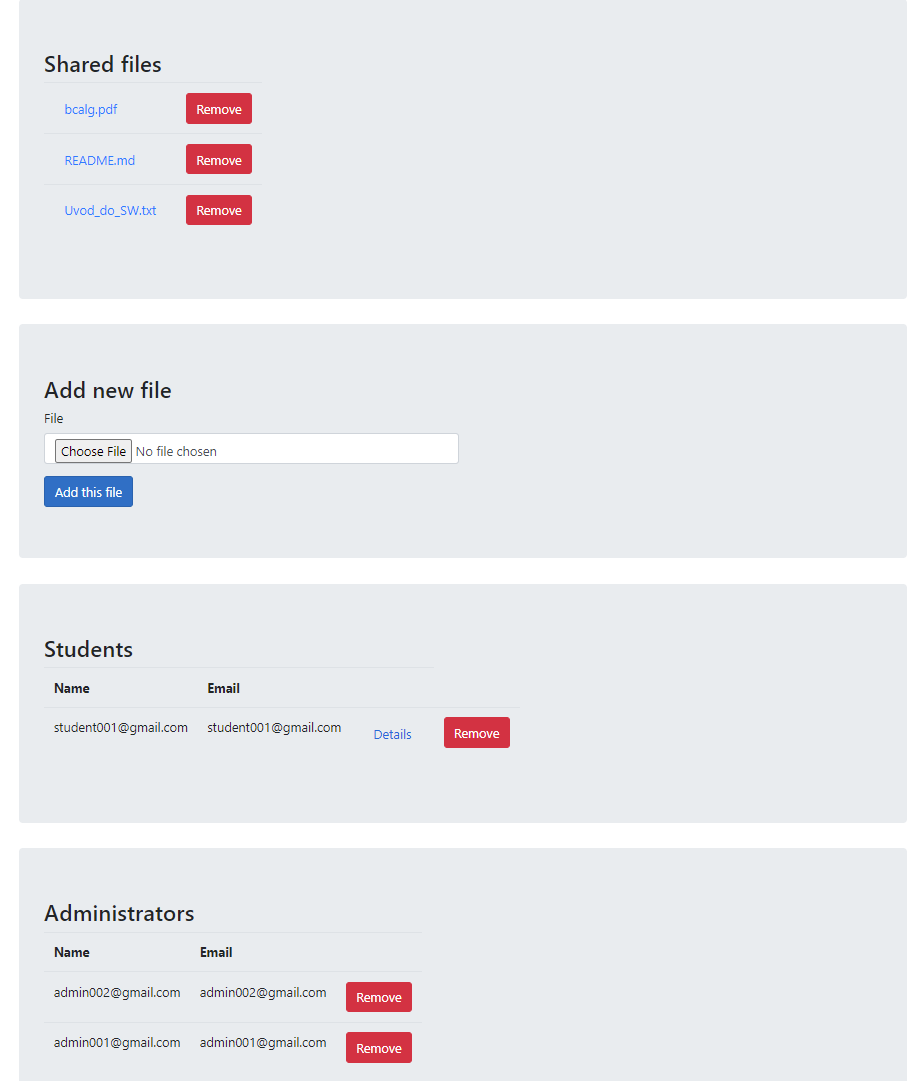
\includegraphics[width=\textwidth]{components_example.PNG}
	\caption{Příklad UI s využitím komponent}
\end{figure}

Na obrázku vidíme část UI s využitím několika komponent. Každá komponenta reprezentuje jeden logický celek uživatelského rozhraní. Konkrétně ve výše uvedeném příkladu máme tyto komponenty

\begin{itemize}
	\item Komponenta se seznamem souborů + formulářem pro přidání souboru
	\item Seznam studentů
	\item Seznam administrátorů
\end{itemize}

Šablona je typicky napsaná v HTML, zatímco backend komponenty je v jazyce Typescript. 

\lstset{style=typescript}
\begin{lstlisting}
@Component({
	selector: 'app-student-list',
	templateUrl: './student-list.component.html',
	styleUrls: ['./student-list.component.css']
})
export class StudentListComponent implements OnInit {

	@Input()
	private courseId: string;
	
	/**
	* list of students
	*/
	public students: CourseMemberOrAdminVM[] = [];
	
	private readonly courseService: CourseService;
	
	constructor(courseService: CourseService) {
		this.courseService = courseService;
	}
	
	ngOnInit() {
		this.courseService.getAllMembers(this.courseId)
		.subscribe(result => {
				this.students = result;
		});
	}
}
\end{lstlisting}

Na výše uvedeném příkladu vidíme, že backend komponenty je klasická Typescript třída označená anotací @Component. U anotace je zároveň uvedený selektor, což je jméno HTML elementu, který slouží k vykreslení komponenty, a umístění souboru se šablonou a CSS styly.

Komponenty typicky používají služby k získání dat z API, podobně jako v příkladu. Můžeme si všimnout, že právě zde probíhá volání metody subscribe, pomocí které v tomto případě data uložíme do proměnné students.

Veřejné položky (například pole students) jsou pak dostupné v HTML šabloně. Některé položky (například courseId) jsou označené anotací @Input, která označuje parametry šablony.

Pro ilustraci uvedeme také šablonu komponenty:

\lstset{style=html}
\begin{lstlisting}
<div class="jumbotron">
	<h3>Students</h3>
	<table class="table table-striped table-responsive">
		<tr>
			<th>Name</th>
			<th>Email</th>
			<th></th>
		</tr>
		<tr *ngFor="let person of students">
			<td>{{person.name}}</td>
			<td>{{person.email}}</td>
			<td>
				<a class="nav-link" routerLink="/students/{{person.id}}">Details</a>
			</td>
		</tr>
	</table>
</div>
\end{lstlisting}

Toto je šablona, která přísluší komponentě StudentListComponent, jenž slouží k zobrazení členů kurzu. Vidíme, že se jedná o klasické HTML, do kterého můžeme vkládat proměnné z backend části komponenty.
Mezi složené závorky vložíme proměnnou, jež chceme vypsat, a framework Angular se sám postará o dosazení příslušné hodnoty.

Můžeme si všimnout atributu *ngFor u elementu <tr>. Takto definujeme, že v tabulce bude pro každého studenta samostatný řádek.
Na každém řádku následně vypíšeme jméno, email a odkaz na detail studenta.

\vspace{\baselineskip}

V šablonách komponent můžeme také vykreslovat jiné šablony.

\begin{lstlisting}
<app-test-list [courseId]="courseId" [isCourseAdmin]="isCourseAdmin"></app-test-list>
<app-file-list [courseId]="courseId" [isCourseAdmin]="isCourseAdmin"></app-file-list>
<app-student-list *ngIf="isCourseAdmin" [courseId]="courseId"></app-student-list>
...
\end{lstlisting}

Na tomto příkladu vidíme kus kódu ze šablony komponenty CourseDetailsComponent, která slouží k zobrazení informací o daném kurzu. Šablona tedy na daném místě vykreslí příslušné šablony (v tomto případě komponenty se seznamy testů, souborů a studentů).

Při volání šablon můžeme také uvést parametry (například parametr courseId v šabloně dané selektorem app-test-list). Tato hodnota se pak uloží do příslušné položky, která je označená anotací @Input, v dané komponentě. To znamená, že komponenta se selektorem app-test-list má položku courseId, která je označená anotací @Input. Pro lepší představu ještě uvedeme kód třídy s komponentou:

\lstset{style=typescript}
\begin{lstlisting}
@Component({
	selector: 'app-test-list',
	templateUrl: './test-list.component.html',
	styleUrls: ['./test-list.component.css']
})
export class TestListComponent implements OnInit, OnChanges {

	@Input()
	public courseId: string;
	...
\end{lstlisting}

\vspace{\baselineskip}

Vzhled stránky se u některých komponent liší podle toho, v jaké je uživateli roli. Můžeme tedy mít komponenty nebo kusy HTML kódu, které se zobrazují například pouze administrátorům daného kurzu.
Toto ve většině případů zajistíme pomocí proměnné, podle které poznáme, jestli je aktuální uživatel administrátor.
Pomocí atributu *ngIf pak zajistíme, že daná část kódu se zobrazí pouze vybraným uživatelům.

\begin{lstlisting}
<app-student-list *ngIf="isCourseAdmin" [courseId]="courseId"></app-student-list>
\end{lstlisting}

V tomto příkladu používáme proměnnou isCourseAdmin, a pomocí atributu *ngIf zajistíme, že komponenta určená selektorem app-student-list se zobrazí pouze administrátorům daného kurzu. 

\vspace{\baselineskip}

V komponentách také poměrně často využíváme obousměrný data binding, který je součástí frameworku Angular. Jedná se o techniku, která umožňuje synchronizaci dat mezi HTML a Typescript objekty.

Pokud tedy změníme data v HTML (například pole formuláře), framework se postará o změnu dat příslušné proměnné v backendu komponenty. Naopak, pokud dojde ke změně hodnoty dané proměnné, pak se framework postará o změnu HTML (například upraví text v poli formuláře).

Obousměrný data binding používáme typicky ve formulářích, podobně jako v následujícím příkladu.

\lstset{style=typescript}
\begin{lstlisting}
export class AddGradeComponent implements OnInit {
	/**
	* grade that we will add to the student
	*/
	public gradeToAdd: AddGradeVM;
	...
}
\end{lstlisting}

Toto je komponenta, která slouží k přidávání známek. 

\lstset{style=html}
\begin{lstlisting}
...
<div class="form-group col-md-2">
	<label for="addGradeForm_Value">Score in %</label>
	<input type="number" min="0" class="form-control" name="value" id="addGradeForm_Value" required
	[(ngModel)]="gradeToAdd.percentualValue">
</div>
<div class="form-group col-md-2">
	<label for="addGradeForm_Weight">Weight</label>
	<input type="number" min="0" class="form-control" name="weight" id="addGradeForm_Weight" required
	[(ngModel)]="gradeToAdd.weight">
</div>
...
\end{lstlisting}

V šabloně pak máme (mimo jiné) políčka formuláře pro procentuální hodnotu a váhu známky.
Pomocí atributu [(ngModel)] nastavíme proměnnou pro data binding. 

Pokud tedy například změníme ve formuláři váhu známky, dojde automaticky ke změně hodnoty gradeToAdd.weight. Podobně, pokud dojde v kódu ke změně hodnoty proměnné gradeToAdd.weight, framework automaticky upraví hodnotu ve formuláři.

Ke stylování elementů používáme framework Bootstrap. 

\newpage

\subsection{Routing}

Frontend část aplikace mimo jiné provádí také routing. Samotný router je součástí frameworku Angular, nicméně potřebujeme nějak nakonfigurovat, jaká komponenta se zobrazí při dotazu na danou URL.

Tato konfigurace se nachází v souboru app.module.ts.
\lstset{style=typescript}
\begin{lstlisting}
RouterModule.forRoot([
	{path: '', component: HomeComponent, pathMatch: 'full'},
	{path: 'students/:id', component: StudentDetailComponent},
	{path: 'courses', component: CourseListComponent},
	...
\end{lstlisting}

V konfiguraci máme vždy uvedenou cestu, a komponentu, která se zobrazí.
Vidíme tedy, že na výchozí stránce bude komponenta HomeComponent. 
Druhý řádek nám říká, že při zadání URL "http://host/students/id", kde id je parametr, se zobrazí komponenta StudentDetailComponent. K parametru id se poté můžeme dostat v komponentě.
Poslední řádek definuje, že na stránce "http://host/courses" se zobrazí CourseListComponent.

\newpage

\section{Zajímavé problémy}

\subsection{ViewModels x DB entity}

Použil jsem různé objekty pro databázové entity a view-modely.

TODO: pořádně rozepsat + vysvětlit + ukázka kódu

\subsection{ViewModels v serverové i klientské části}

view-modely jsou v serverové i klientské části aplikace

TODO: pořádně rozepsat + vysvětlit + ukázka kódu
